% Created 2023-10-09 Mon 12:03
% Intended LaTeX compiler: pdflatex
\documentclass[12pt, a4paper]{article}
\usepackage[utf8]{inputenc}
\usepackage[T1]{fontenc}
\usepackage{graphicx}
\usepackage{longtable}
\usepackage{wrapfig}
\usepackage{rotating}
\usepackage[normalem]{ulem}
\usepackage{amsmath}
\usepackage{amssymb}
\usepackage{capt-of}
\usepackage{hyperref}
\usepackage{placeins}
\usepackage{gensymb}
\usepackage[letterpaper]{geometry}
\geometry{top=1.0in, bottom=1.0in, left=1.0in, right=1.0in}
\usepackage{rotating}
\usepackage{graphicx}
\usepackage{pgfplots}
\usepackage{filecontents}
\usepackage{tikz}
\usepackage{fancyhdr}
\usepackage{enumitem}
\pagestyle{fancy}
\lhead{}
\chead{}
\rhead{Johnson \thepage}
\lfoot{}
\cfoot{}
\rfoot{}
\renewcommand{\headrulewidth}{0pt}
\renewcommand{\footrulewidth}{0pt}
\setlength\headsep{0.333in}
\newcommand{\bibent}{\noindent \hangindent 40pt}
\newenvironment{workscited}{\newpage \begin{center} Works Cited \end{center}}{\newpage }
\graphicspath{ {./attachments/} }
\author{Christian}
\date{\today}
\title{}
\hypersetup{
 pdfauthor={Christian},
 pdftitle={},
 pdfkeywords={},
 pdfsubject={},
 pdfcreator={Emacs 28.2.50 (Org mode 9.7-pre)}, 
 pdflang={English}}
\begin{document}

\begin{document}
\begin{flushleft}
Christian Johnson\\
\vspace{2mm}Dr. Paul Crilly\\
\vspace{2mm}Antennas and Propogation\\
\vspace{2mm}October 09 2023\\
\vspace{4mm}\begin{center}
Lab 4 Report
\end{center}
\vspace{1mm}\setlength{\parindent}{0.5in}

\begin{abstract}
This laboratory exercise focused on the exploration of electromagnetic compatibility and radio frequency interference. Our primary objective was investigating interference suppression, and how high-frequency interferenece can affect lower-frequency signals through shielded cables. We used clip-on ferrite chokes and inductors to mitigate this interference. Employing clip-on ferrite chokes and inductors yielded a promising decrease in interference. From our results, using two chokes in tandem seemd to be the most effective, but this will change based on the system in question. There will always be some break point, past which one should notice diminishing returns in attenuation. Similarly, when using inductors, if the system is overdamped, one may start to notice a "ringing" effect, which we found when we used too large of an infuctor. Our findings demonstrate the importance of electromagnetic interference in practical uses, the effectiveness of chokes in mitigating that interference, and the importance of choosing the right mitigation technique for certain scenarios. 
\end{abstract}
\section*{Procedures}
\label{sec:org7da4ef3}
In preparation for this lab, we removed the shield from a 12" piece of RG-213 COAX, attaching an Aphenol BNC connector to one end. At the other end, we exposed a 1/2" section of shield and a 2" inner conductor section, stripping 1/4" off the insulation. Finally, we slid the RG-213 shield over the RG-58 COAX and soldered a 4" hookup wire to the end of the shield, near the BNC connector.
After verifying our square wave output, we connected our RG-58 cable (with the RG-213 shield) to a 20 MHz sine wave generator, and the square wave generator on our oscilloscope. We attached our scope leads to the shielding, lead cable, and RG-58, seeking to observe the interference induced on the square wave by the 20 MHz signal. Next, we tried using 1, then 2 "clip-on" iron chokes, attaching them to the RG-58 wire and observing their effects. Our final step was to replace the clip-on chokes with \(1\mu F\) then \(10mF\) inductors.
\section*{Results}
\label{sec:org7ecc56c}
We began by recording the interference with no chokes or inductors, noting \(\Delta Y\) of -800mV at 1\(V_{pp}\), and \(\Delta Y\) of 1.925V at 2.5\(V_{pp}\).
After adding a single choke, the interference decreased noticeably - \(\Delta Y\) falling to -375mV at 1V. After adding a second choke, we then interference decreased less noticeably than with a single choke, \(\Delta Y\) falling to -262.5mV at \(1V_{pp}\) with an attenuation of -9.679 dB, and 500mV at \(2.5V_{pp}\) with an attenuation of -11.709 dB. As we added more chokes, we noticed increasingly diminishing returns, with 2 chokes seeming to be the most effective and practical solution. With more than 2 chokes, we saw almost no change in the noise reduction across the line.
We added the inductors next, wiring them in series between the lead lines and the coax cable. At \(2.5V_{pp}\), the signal exhibited \(\Delta Y\) of 1.787V without an inductor. The \(1\mu H\) inductor reduced this to 937.5mV, not performing quite as well as either one or two chokes, but serving as a relatively effective method to reduce interference. After adding a \(10mH\) inductor, we noticed an interesting effect, with the upper level of the square wave peaking at the forward edge, before falling back to level at the trailing edge. This phenomenon, known as ringing, consists of a series of over and under shoots and typically occurs after a signal undergoes a sudden change.
\section*{Conclusions}
\label{sec:orgff358df}
Our experimentation revealed significant insights into methods to reduce interference. Using clip-on ferrite chokes, we observed a clear reduction in interference, with two chokes providing optimal results for both 1V and 2.5V peak to peak signals at 20 MHz. However, it is essential to note that increasing the number of chokes did not proportionally increase attenuation, demonstrating substantially diminishing returns past a certain point. Additionally, we explored the impact of inductors on interference reduction. A \(1\mu H\) inductor effectively reduced interference, however, when a \(10mH\) inductor was introduced, we observed undesirable amounts of ringing. These findings emphasize the importance of selecting the most suitable interference mitigation technique based on specific requirements and signal characteristics. 




\newpage
\begin{center}
Appendices
\end{center}
\begin{figure}[htb]
\centering
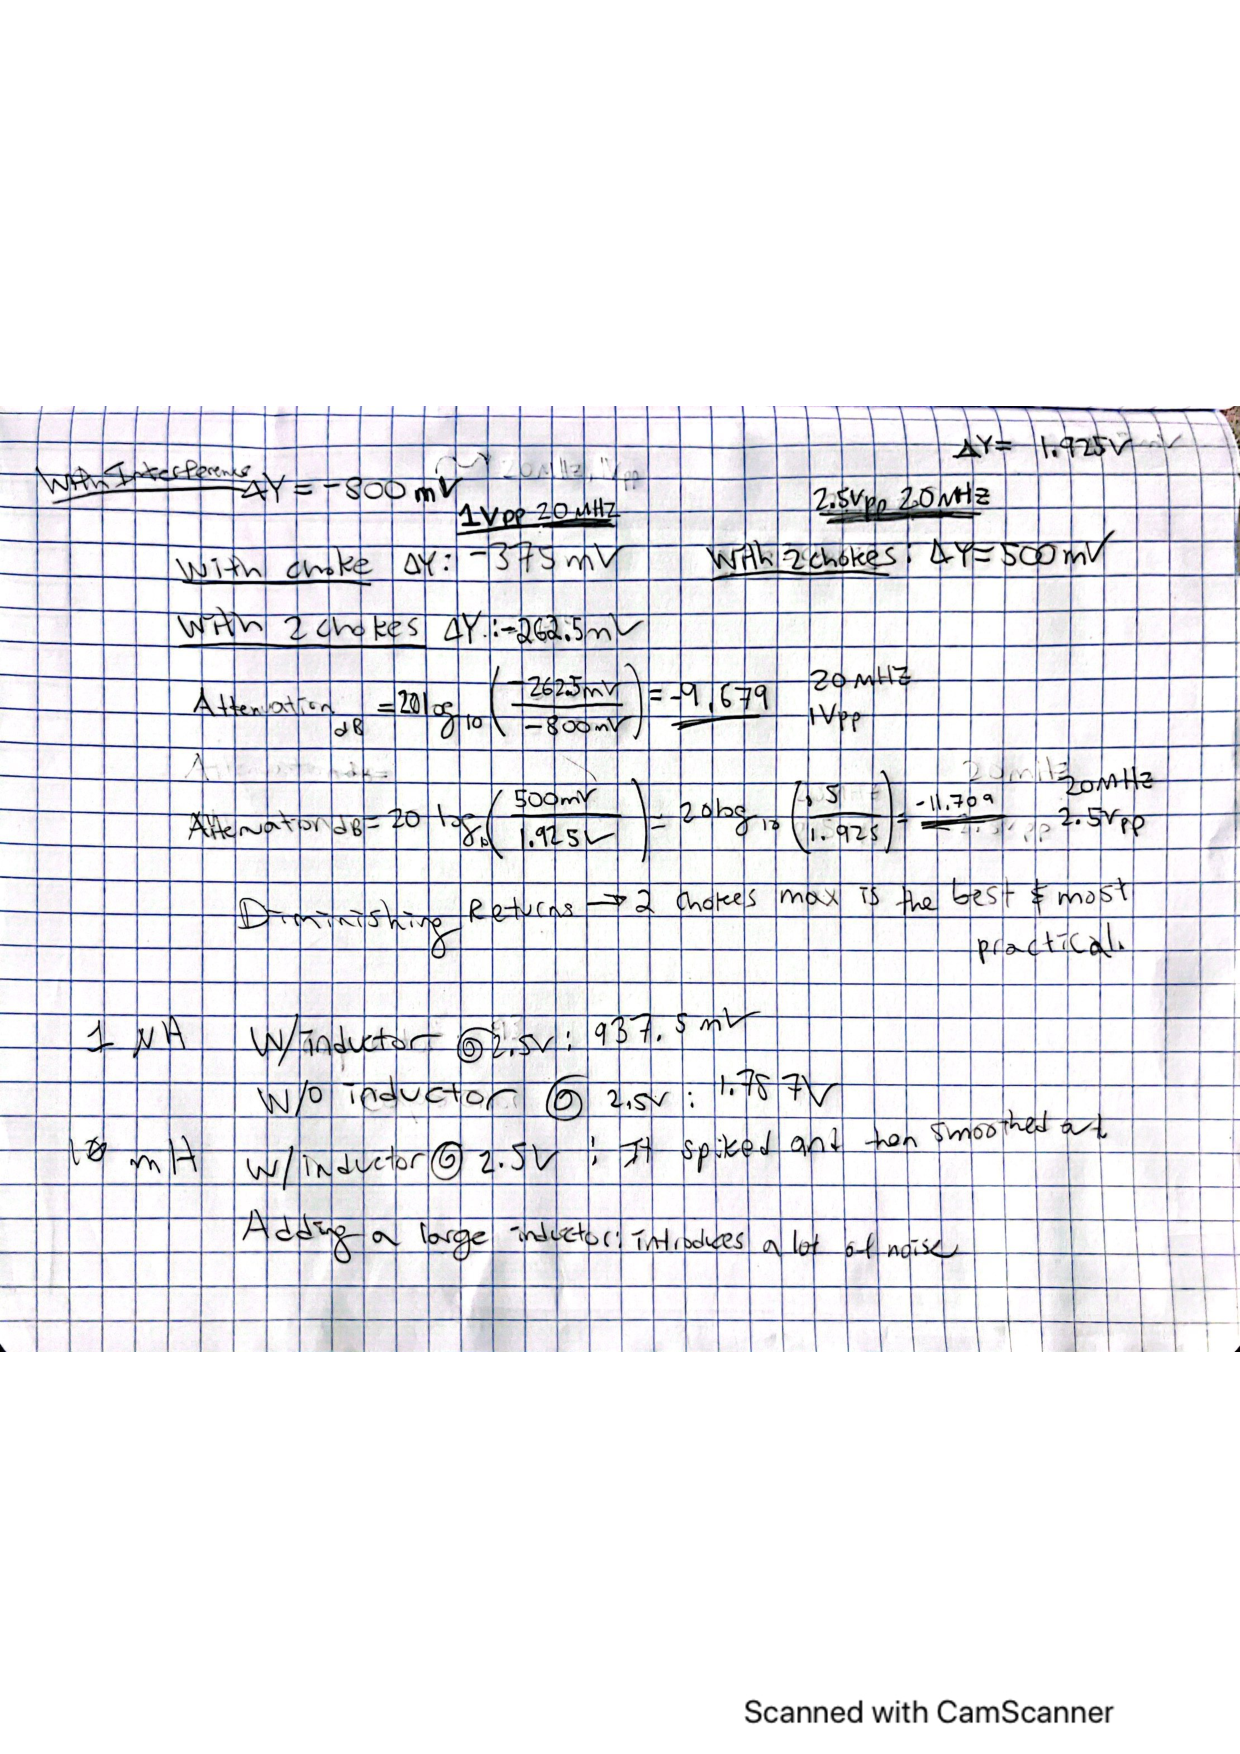
\includegraphics[width=0.7\textwidth]{LabNotebook.pdf}
\caption{Lab Notebook}
\end{figure}
\newpage

\begin{center}
Lab Questions
\end{center}
\vspace{2mm}
\begin{enumerate}[label=\textbf{\arabic*.}]
\item What was the most effective choke configuration? Which added the most attenuation?
We noticed the greatest amount of attenuation (-9.679 dB) with 2 chokes in series.
\item State analytically why a choke will reduce interference.
A choke reduces interference because of its impedance. It introduces high impedance to high frequency components of a signal. The inductive impedance of the choke will increase with frequency, effectively blocking the high frequency interference and letting the lower frequency components pass. 
\item What are the advantages and diadvantages of the two reduction methods that you tested?
Clip-on ferrites are signigicantly easier to install, making them more practical, but they may not provide the same precision afforded by an inductor. In contrast, since an inductor must be installed in series to the cable, it is significantly more difficult to implement, and may distort the signal shape (as we saw in the latter part of our experiment), but can be far more precise. 
\item Where else have clip on ferrite cores been used to reduce interference?
Clip in ferrite cores are typically used on power supply cables for consumer electronics to help reduce the impact of power surges or other variance in the supply of power to the device (almost every laptop computer includes a ferrite core just before the pc end of the plug, after the adapter/transformer/I'm not sure what the big brick is actually called). 
\item Is there a difference between a choke and an inductor?
A choke is a specific type of inductor, used to block high frequency signals and interference, while inductor is a much more general term. 
\item Why could a choke distort the shape of a square wave and not a sine wave?
Since square waves are constructed of multiple harmonics, layered to produce the sharp edges that we see, when this signal passes through a choke, it can affect the higher pitched harmomics more than those closer to the fundamental frequency, causing the square wave to change shape. Sine waves on the other hand ARE the fundamental frequency - they are a solitary signal where square waves are a compound product of many. Because of this, the chokes effect is more "balanced" since there is only one frequency for it to affect. (I had to google this, because I didn't really understand how square waves are produced - still not sure I fully grasp it)
\item Is noise different from interference? How?
Interference is when a signal is corrupted by a deterministic (man-made) source - such as another signal. Noise however, is non-deterministic. It is random and almost always unwanted. Interference has a single (or multiple) unique source(s), while noise is a function of mean and standard deviation. 
\item Aside from chokes or inductors, how else could we attenuate the 20 MHz signal, without affecting the 1 kHz waveform?
Without using chokes or inductors, we could implemebt a low-pass filter. A properly designed filter would allow lower frequency signal components to pass, while attenuating anything above a certain point. 
\item Why would degree of attenuation be affected by the voltage through the cable?
The degree of attenuation can be affected by the voltage because it influences the amplitude of the interference signal (relative to the original signal). When the interference signal is signigicantly smaller than the original, the attenuation may appear more significant.
\end{enumerate}

\end{document}
\end{document}